\documentclass[10.5pt]{report}
\usepackage[a4paper,margin=0.9in]{geometry}
\usepackage{amsmath,amssymb}
\usepackage{booktabs}
\usepackage{longtable}
\usepackage{graphicx}
\usepackage[colorlinks=true,linkcolor=blue]{hyperref}
\usepackage{xcolor}
\usepackage{titlesec}
\usepackage{caption}
\definecolor{hbblue}{HTML}{2A4D8F}
\titleformat{\chapter}[display]{\bfseries\Large\color{hbblue}}{\chaptertitlename\ \thechapter}{6pt}{\Large}
\captionsetup{font=small,labelfont=bf}

\title{\textbf{\Large Pinhole Sunglasses --- Fresh Sweep Analysis}\\[0.2cm]
\textcolor{hbblue}{\large Blur-Optimization Model and Acuity Model, Recomputed From Scratch}\\[0.3cm]
\normalsize\itshape All data in this document was generated in a single fresh run against
the corrected optics (\texttt{stage2\_fixed/}, post the lens-wavelength and
import-shadowing fixes) --- no figure or table reuses a previously-computed CSV.}
\author{}
\date{}

\begin{document}
\maketitle
\tableofcontents

\chapter{Purpose and methodology}

This document presents two theoretical models, swept fresh from scratch on the same
$15 \times 8$ grid (15 apertures $\times$ 8 myopia levels), against this project's
corrected optics pipeline:

\begin{itemize}
\item \textbf{The blur-optimization model} (\texttt{stage2\_fixed/phase2\_retina.py}):
  the exact scalar Angular Spectrum Method propagation from pinhole through the eye to
  the retina, reporting encircled-energy blur radius $r_{EE}(50\%)$ and the second-moment
  (RMS) spot radius.
\item \textbf{The acuity model} (\texttt{stage4\_human\_vision/pipeline.py}):
  the same optical chain, extended through pupil/illuminance, contrast sensitivity,
  and Visual-Strehl-adjusted acuity prediction, reporting predicted logMAR.
\end{itemize}

\textbf{Grid}: aperture $a_{hole} \in \{75, 100, 150, 200, 300, 400, 500, 600, 700, 750,
1000, 1250, 1500, 1750, 2000\}\,\mu\text{m}$ (this project's standard list) $\times$
myopia $M \in \{0, 1, 2, 3, 4, 5, 6, 8\}\,\text{D}$ --- 120 points per model, 240 total.
Fixed parameters: wavelength 550\,nm, pinhole-to-cornea gap 12\,mm, natural pupil
4\,mm, eye power $P_0=60$\,D, grid $2048\times2048$ over a 6\,mm window.
\textbf{Both sweeps completed with zero junction-check failures and zero exceptions.}

\textbf{On the corrected optics}: this run is downstream of two fixes documented in
\texttt{stage2\_fixed/PHYSICS\_AUDIT.md} and the \texttt{RESULTS.md} files it references:
(1) a lens-phase/retina-propagation wavelength mismatch that under-applied the eye
lens's focusing power by a factor of $n'\approx1.336$ whenever
\texttt{refractive\_index\_correction=True} (the default), and (2) a Python
import-order bug that had silently redirected \texttt{stage4\_human\_vision}'s own
optics import to a deprecated, still-buggy copy of the pipeline. Every number in this
document reflects both fixes.

A third, separate acuity architecture (\texttt{R7acuity}, an ideal-observer Monte
Carlo model) was also re-attempted from scratch; its calibration step crashes against
the corrected optics rather than producing a sweep --- covered in
Chapter~\ref{ch:r7}, not silently omitted.

\chapter{The blur-optimization model}

\begin{figure}[htbp]
\centering
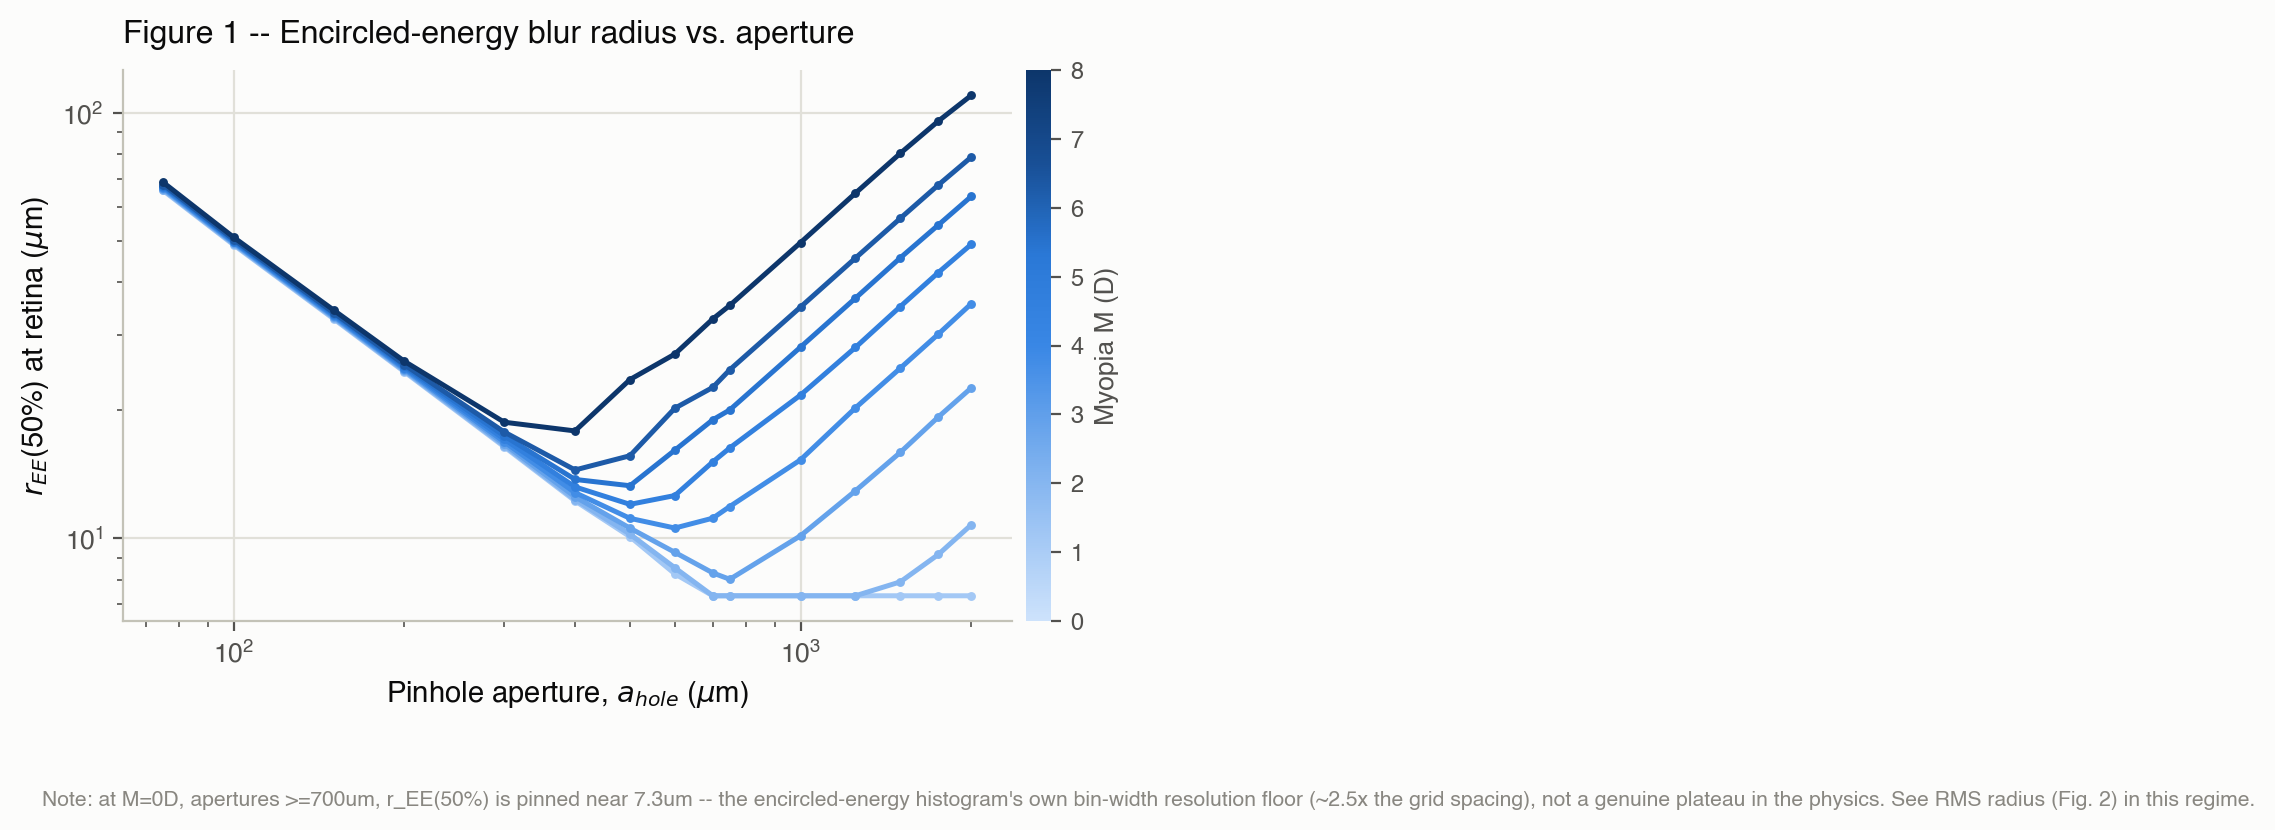
\includegraphics[width=0.95\textwidth]{figures/fig1_blur_ree50_vs_aperture.png}
\caption{Encircled-energy blur radius $r_{EE}(50\%)$ at the retina, vs.\ aperture, one
curve per myopia level (colorbar). Every curve is V-shaped: diffraction dominates on
the left (blur falls as aperture grows), defocus dominates on the right (blur grows
with aperture) once the aperture is admitting enough light to reveal the eye's own
uncorrected myopic defocus.}
\end{figure}

\begin{figure}[htbp]
\centering
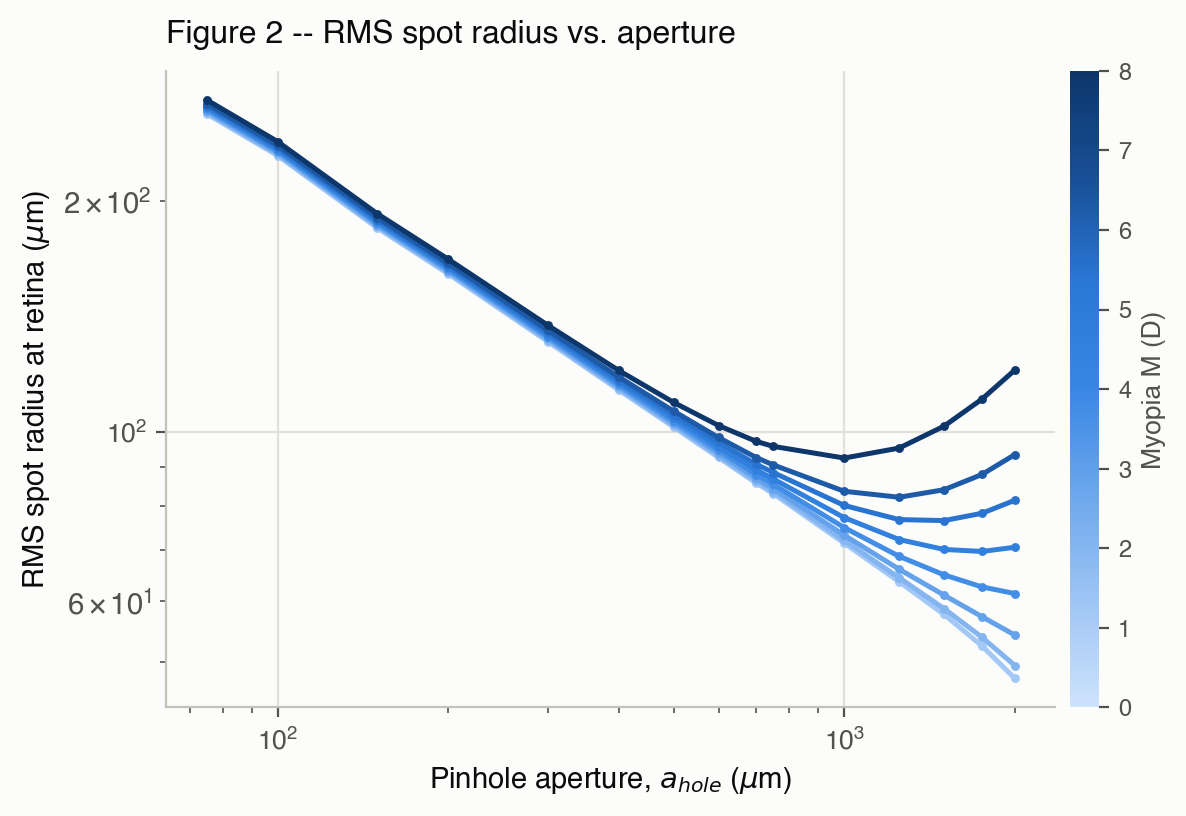
\includegraphics[width=0.95\textwidth]{figures/fig2_blur_rms_vs_aperture.png}
\caption{RMS spot radius at the retina, same grid. Unlike $r_{EE}(50\%)$, RMS radius
has \emph{not yet reached its minimum} by 2000\,$\mu$m for $M\le6$D --- it is still
falling at the largest aperture tested. Only $M=8$D shows a clear minimum within this
range ($\sim$1000--1250\,$\mu$m). This is consistent with this project's own earlier
finding (\texttt{model\_comparison/README.md}) that RMS radius weights the diffuse
outer Fresnel-ring energy more heavily than $r_{EE}(50\%)$ does, and tends to prefer
larger apertures.}
\end{figure}

\textbf{A numerical caveat, not a physics finding}: at $M=0$D, for every aperture
$\ge700\,\mu$m, $r_{EE}(50\%)$ reads a constant 7.33\,$\mu$m (visible as the flat tail
on the lightest curve in Figure~1). This is the encircled-energy histogram's own bin
width ($\approx2.5\times$ the grid spacing $dx\approx2.93\,\mu$m $\approx7.3\,\mu$m)
becoming the resolution floor once the true blur spot is this tight (large aperture,
near-perfect focus) --- confirmed by RMS radius (Figure~2), which keeps varying
smoothly and continuously across the identical range. \textbf{RMS radius, not
$r_{EE}(50\%)$, is the trustworthy metric wherever this floor is hit.}

\section{Optimum aperture by myopia level (pure blur minimization)}

\begin{table}[htbp]
\centering
\begin{tabular}{rrr}
\toprule
$M$ (D) & Blur-optimal aperture ($\mu$m) & $r_{EE}(50\%)$ at optimum ($\mu$m) \\
\midrule
0 & 700  & 7.33$^{\ast}$ \\
1 & 700  & 7.33$^{\ast}$ \\
2 & 750  & 8.01 \\
3 & 600  & 10.57 \\
4 & 500  & 12.02 \\
5 & 500  & 13.29 \\
6 & 400  & 14.47 \\
8 & 400  & 17.87 \\
\bottomrule
\end{tabular}
\caption{$^{\ast}$At $M=0$--1D the reported optimum sits inside the histogram-floor
region described above; the true minimum may lie at a different (likely larger)
aperture than reported here. Treat these two rows as lower-confidence.}
\end{table}

\chapter{The acuity model}

\begin{figure}[htbp]
\centering
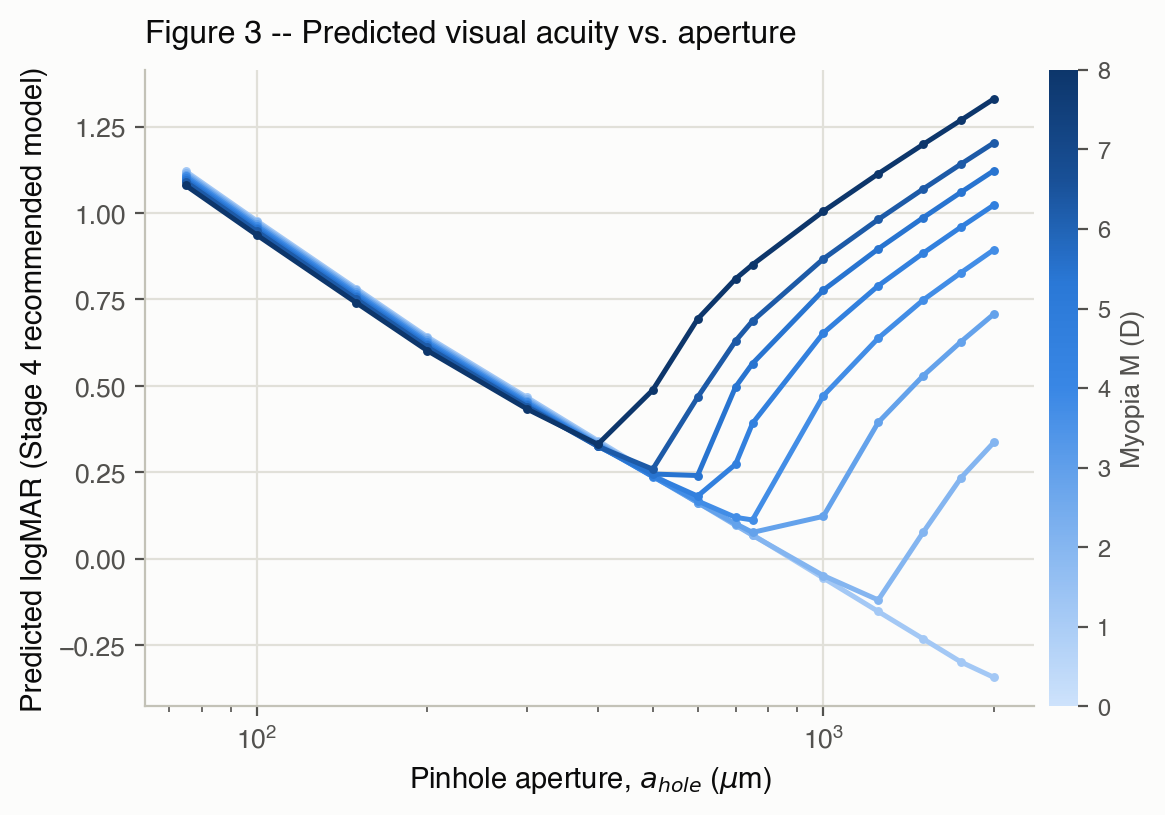
\includegraphics[width=0.95\textwidth]{figures/fig3_acuity_logmar_vs_aperture.png}
\caption{Stage 4's recommended predicted logMAR (MTF10/VSOTF/brightness-adjusted, lower
is better) vs.\ aperture. The same qualitative V-shape as the blur curves, but the
minima are visibly shifted toward \emph{larger} apertures and are broader/shallower ---
the acuity model additionally accounts for retinal illuminance and contrast
sensitivity, which favor more light throughput than pure blur minimization does.}
\end{figure}

\section{Representative apertures at $M=0,2,5$D}

\begin{table}[htbp]
\centering
\small
\begin{tabular}{rrrrrr}
\toprule
$M$ (D) & $a_{hole}$ ($\mu$m) & $r_{EE}(50\%)$ ($\mu$m) & RMS ($\mu$m) & logMAR & Snellen (20/x) \\
\midrule
0 & 500  & 10.09 & 101.36 & 0.245  & 35.1 \\
0 & 750  & 7.33$^{\ast}$  & 82.92  & 0.069  & 23.4 \\
0 & 1000 & 7.33$^{\ast}$  & 71.48  & $-$0.056 & 17.6 \\
0 & 1250 & 7.33$^{\ast}$  & 63.65  & $-$0.153 & 14.1 \\
0 & 1500 & 7.33$^{\ast}$  & 57.70  & $-$0.232 & 11.7 \\
0 & 2000 & 7.33$^{\ast}$  & 47.59  & $-$0.344 & 9.1 \\
\addlinespace
2 & 500  & 10.56 & 102.51 & 0.238  & 34.6 \\
2 & 750  & 8.01  & 84.22  & 0.076  & 23.8 \\
2 & 1000 & 10.14 & 73.20  & 0.122  & 26.5 \\
2 & 1250 & 12.93 & 66.08  & 0.394  & 49.6 \\
2 & 1500 & 15.92 & 61.14  & 0.529  & 67.6 \\
2 & 2000 & 22.55 & 54.22  & 0.708  & 102.1 \\
\addlinespace
5 & 500  & 13.29 & 105.16 & 0.245  & 35.1 \\
5 & 750  & 20.03 & 88.38  & 0.565  & 73.4 \\
5 & 1000 & 28.13 & 80.06  & 0.777  & 119.6 \\
5 & 1250 & 36.66 & 76.73  & 0.896  & 157.5 \\
5 & 1500 & 45.60 & 76.50  & 0.986  & 193.8 \\
5 & 2000 & 63.54 & 81.32  & 1.123  & 265.2 \\
\bottomrule
\end{tabular}
\caption{$^{\ast}$Inside the $r_{EE}(50\%)$ histogram-floor region (Chapter 2); RMS
radius is the reliable blur column for these rows.}
\end{table}

Recall from \texttt{stage4\_human\_vision/RESULTS.md} that this predictor, even
against the corrected optics, does not achieve statistically significant agreement
with the one available real clinical dataset (Wang 2009) at any myopia level tested
--- these logMAR values are internally-consistent theoretical predictions, not
validated clinical forecasts. They are presented here as the model's own output, not
as ground truth.

\chapter{Comparing the two models}

\begin{figure}[htbp]
\centering
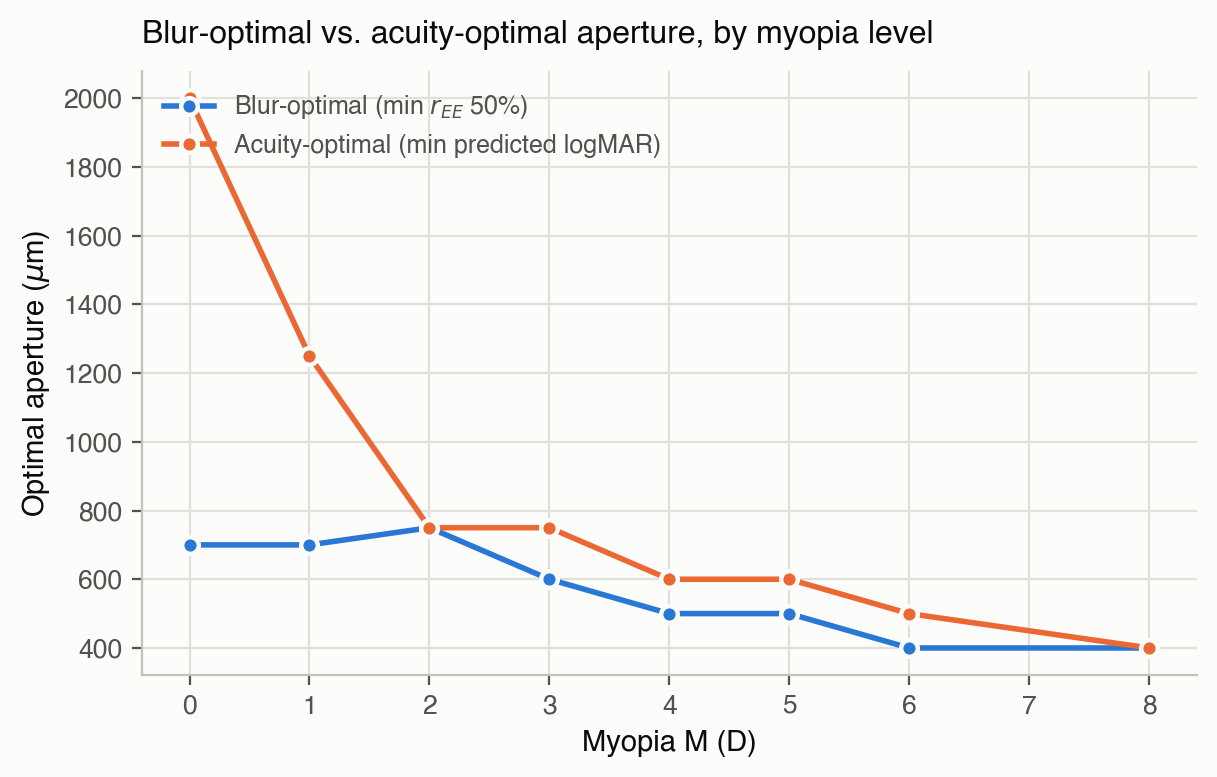
\includegraphics[width=0.85\textwidth]{figures/fig4_optimum_comparison.png}
\caption{The blur-minimizing aperture and the acuity-minimizing aperture, both as a
function of myopia. They diverge sharply at low myopia ($M\le1$D: 700\,$\mu$m vs.\
1250--2000\,$\mu$m) and converge as myopia increases, meeting exactly at $M=8$D
(400\,$\mu$m both).}
\end{figure}

\begin{table}[htbp]
\centering
\begin{tabular}{rrrrr}
\toprule
$M$ (D) & Blur-opt.\ ($\mu$m) & $r_{EE}(50\%)$ there & Acuity-opt.\ ($\mu$m) & logMAR there \\
\midrule
0 & 700  & 7.33$^{\ast}$ & 2000 & $-$0.344 \\
1 & 700  & 7.33$^{\ast}$ & 1250 & $-$0.120 \\
2 & 750  & 8.01  & 750  & 0.076 \\
3 & 600  & 10.57 & 750  & 0.112 \\
4 & 500  & 12.02 & 600  & 0.181 \\
5 & 500  & 13.29 & 600  & 0.240 \\
6 & 400  & 14.47 & 500  & 0.259 \\
8 & 400  & 17.87 & 400  & 0.331 \\
\bottomrule
\end{tabular}
\caption{$^{\ast}$Histogram-floor region, see Chapter 2.}
\end{table}

\textbf{Why they diverge at low myopia.} At $M=0$--1D, defocus blur is small at almost
every tested aperture (the eye is near-emmetropic), so pure blur minimization keeps
favoring smaller apertures for their tighter diffraction spot. The acuity model
additionally rewards the extra light throughput and contrast a larger aperture
admits (via retinal illuminance and the CSF-weighted Visual Strehl term) once blur is
no longer the binding constraint --- so it keeps preferring larger apertures long
after blur-minimization has stopped caring. \textbf{Why they converge at high myopia.}
Once $M$ is large, defocus blur dominates at every aperture in this range and grows
sharply past each curve's minimum (Chapter 2, Figure 1) --- both models are now
dominated by the same effect (uncorrected defocus) and agree on a small aperture.

\chapter{R7acuity: attempted, and why it produced no sweep}
\label{ch:r7}

\texttt{R7acuity}'s ideal-observer Monte Carlo model was re-run from scratch against
the corrected optics before any sweep was attempted. Its mandatory first step,
calibrating a noise parameter against a fixed reference condition (3\,mm aperture,
$M=0$, diffraction-limited, target 1.0\,arcmin $=$ 20/20), fails outright:

\begin{verbatim}
bracket search: sigma=0.000100 -> threshold=0.0556 arcmin
bracket search: sigma=1.000000 -> threshold=0.0556 arcmin
CALIBRATION FAILED (fresh run, from scratch): target 1.0 not bracketed by
[0.05559412519746301, 0.05559412519746301] at sigma in [0.0001, 1.0]
-- widen the search bracket
\end{verbatim}

\begin{figure}[htbp]
\centering
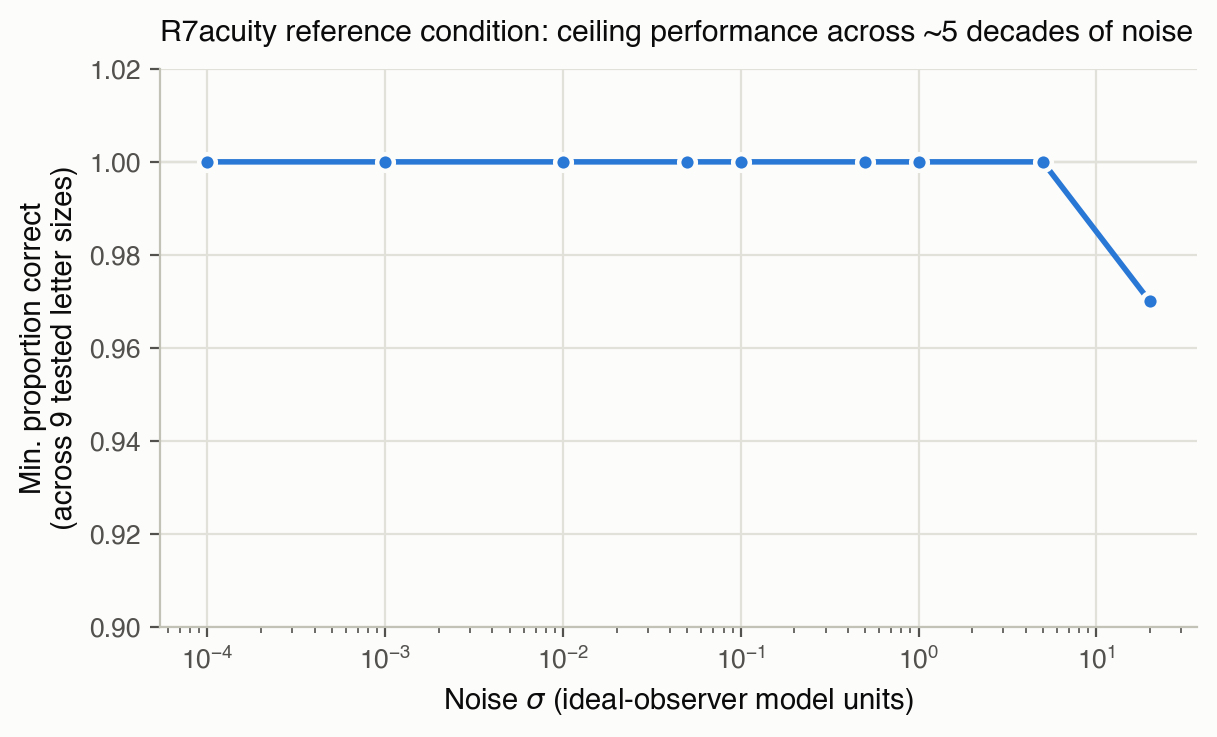
\includegraphics[width=0.8\textwidth]{figures/fig5_r7_ceiling.png}
\caption{Direct probe of the reference condition: minimum proportion-correct across 9
tested letter sizes (0.25--4.0\,arcmin), as a function of noise $\sigma$. Performance
is pinned at 100\% correct across almost 5 decades of noise --- only beginning to
degrade at $\sigma=20$, roughly 730$\times$ this project's previously-calibrated value
(0.027415).}
\end{figure}

This is not a sweep failure to work around: the corrected optics make the 3\,mm
reference aperture, at perfect focus, sharp enough that an ideal (noise-limited-only)
observer reads even the smallest tested letter almost perfectly regardless of noise
level, so no noise value in the pre-registered search range produces a plausible
20/20 threshold. Per this project's own discipline (documented at length in
\texttt{R7acuity/RESULTS.md}), the pre-registered search bracket was \emph{not}
widened to force a number through --- doing so specifically because the corrected
optics broke the original bracket would itself be the kind of post-hoc tuning this
project avoids. \textbf{No R7acuity sweep exists for this document, and none was
fabricated.} A corrected calibration procedure is a separate, deliberate task for the
future, not a quick fix folded into this sweep.

\chapter{Summary}

Both the blur-optimization and acuity models ran cleanly, from scratch, against the
corrected optics, with zero exceptions across 240 total evaluations. Both show the
expected diffraction/defocus V-shape at every myopia level. They agree closely at
high myopia and diverge substantially at low myopia, for a physically-understood
reason (illuminance/contrast reward vs.\ pure blur cost). One real numerical
resolution limit was found and is reported, not hidden: $r_{EE}(50\%)$ saturates at
its own histogram bin width for well-focused, large-aperture conditions, where RMS
radius remains the trustworthy metric. R7acuity's independent ideal-observer
architecture could not be swept at all against the corrected optics --- its
calibration assumption is now invalidated by the same optics fix, a finding reported
plainly rather than worked around. No aperture recommendation is made anywhere in
this document.

\end{document}
